\documentclass[tikz,border=10pt]{standalone}
\begin{document}
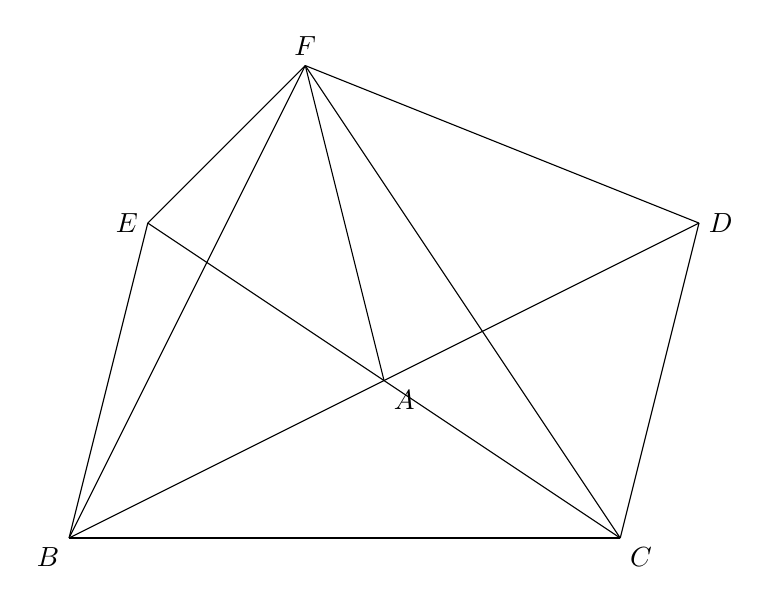
\begin{tikzpicture}
    \coordinate (B) at (0,0);
    \coordinate (C) at (7,0);
    \coordinate (F) at (3,6);
    \coordinate (A) at (4,2);
    \coordinate (D) at (8,4);
    \coordinate (E) at (1,4);

    \draw (B) -- (C);
    \draw (C) -- (D);
    \draw (D) -- (F);
    \draw (F) -- (E);
    \draw (E) -- (B);
    \draw (B) -- (F);
    \draw (C) -- (F);
    \draw (B) -- (D);
    \draw (C) -- (E);
    \draw (F) -- (A);

    \node[below left] at (B) {$B$};
    \node[below right] at (C) {$C$};
    \node[above] at (F) {$F$};
    \node[below right] at (A) {$A$};
    \node[right] at (D) {$D$};
    \node[left] at (E) {$E$};
\end{tikzpicture}
\end{document}
